\documentclass[defaultstyle,10pt,master,Helvetica]{thesis}
%% Enable Latin characters
\usepackage[utf8]{inputenc}
%% Better equations
\usepackage{amsmath, amsthm, amssymb, amsfonts}
%% Used for abreviations??
\usepackage{nomencl}
\renewcommand{\nomname}{List of Abbreviations}
\makenomenclature
%% Advanced tables
\usepackage{multirow}
\usepackage{colortbl}
\usepackage{tabularx}                 
\newcommand{\specialcell}[2][c]{%
  \begin{tabular}[#1]{@{}c@{}}#2\end{tabular}}

%% Better figures
\usepackage{graphics}
\usepackage{epsfig}
\usepackage[hang,small,bf]{subfigure}

%% The two packages are not compatible, and you should use one of the two. Notice however that the
\usepackage[square,numbers,sort&compress]{natbib}

%% Acronyms
\usepackage[printonlyused]{acronym}
\usepackage[acronym]{glossaries}

%% Pseudo-code algorithms
\usepackage[]{algorithm2e}

%% Set links for references and citations in document
\usepackage{hyperref}
\hypersetup{ %a4paper=true,
             colorlinks=false,
             citecolor=red,
             breaklinks=true,
             bookmarks=true,
             bookmarksnumbered=true,
             bookmarksopen=true,
             pdftitle={HOMOPHILIC SELF ORGANIZING FEATURE MAPS: FINDING TOPICS ON SOCIALY CONNECTED DATA, USING SOCIAL NETWORK RELATIONS},
             pdfauthor={Bernardo Simões},
             pdfsubject={Thesis - Master Degree},                  
             pdfcreator={Vim - Bernardo Simões},
             pdfkeywords={thesis, topic detection, twitter, self-organizing maps, classification, clustering}
}

\usepackage{booktabs}
%% Set paragraph counter to alphanumeric mode
\renewcommand{\theparagraph}{\Alph{paragraph}~--}

%% Brian stuff, not sure what
\usepackage{float}
\floatstyle{ruled}
\newfloat{formulation}{thp}{lop}
\floatname{formulation}{Formulation}
\usepackage{enumitem}
\setdescription{style=multiline}

%% Page formatting
\hoffset 0in
\voffset 0in
\oddsidemargin 0.71cm
\evensidemargin 0.04cm
\marginparsep 0in
\topmargin -0.25cm
\textwidth 15cm
\textheight 23.5cm

\usepackage{fancyhdr}
\pagestyle{fancy}
\renewcommand{\chaptermark}[1]{\markboth{\thechapter.\ #1}{}}
\renewcommand{\sectionmark}[1]{\markright{\thesection\ #1}}
\fancyhf{} \fancyhead[LE]{\bfseries\nouppercase{\leftmark}}
\fancyhead[RO]{\bfseries\nouppercase{\rightmark}}
\fancyfoot[LE,RO]{\bfseries\thepage}
\renewcommand{\headrulewidth}{0.5pt}
\renewcommand{\footrulewidth}{0.5pt}
\addtolength{\headheight}{2pt} % make space for the rule
\fancypagestyle{plain}{%
   \fancyhead{} % get rid of headers
   \renewcommand{\headrulewidth}{0pt} % and the line
   \renewcommand{\footrulewidth}{0pt}
}
\fancypagestyle{blank}{%
   \fancyhf{} % get rid of headers and footers
   \renewcommand{\headrulewidth}{0pt} % and the line
   \renewcommand{\footrulewidth}{0pt}
}
\fancypagestyle{abstract}{%
   \fancyhead{}
   \renewcommand{\headrulewidth}{0pt}
   \renewcommand{\footrulewidth}{0.5pt}
}
\fancypagestyle{document}{%
	\fancyhf{} \fancyhead[LE]{\bfseries\nouppercase{\leftmark}}
	\fancyhead[RO]{\bfseries\nouppercase{\rightmark}}
	\fancyfoot[LE,RO]{\bfseries\thepage}
	\renewcommand{\headrulewidth}{0.5pt}
	\renewcommand{\footrulewidth}{0.5pt}
	\addtolength{\headheight}{2pt} % make space for the rule
}
\setcounter{secnumdepth} {5}
\setcounter{tocdepth} {5}
\renewcommand{\thesubsubsection}{\thesubsection.\Alph{subsubsection}}

\renewcommand{\subfigtopskip}{0.3 cm}
\renewcommand{\subfigbottomskip}{0.2 cm}
\renewcommand{\subfigcapskip}{0.3 cm}
\renewcommand{\subfigcapmargin}{0.2 cm}


\begin{document}
\pdfbookmark[0]{Titlepage}{Title}
% IST requires the title page to be written in Portuguese
% IST requires the logo to measure 2cm
\univlogo{3cm}{2cm}{images/IST_A_CMYK_POS.eps}

% OPTIONAL: the thesis logo image
%\thesislogo{2.5cm}{6cm}{images/thesis_logo.eps}

\title{HOMOPHILIC SELF ORGANIZING FEATURE MAPS: FINDING TOPICS ON SOCIALY CONNECTED DATA, USING SOCIAL NETWORK RELATIONS}

\author{Bernardo Simões}
\degree{Engenharia de Redes de Comunicações}
% \otherdegree{Mestre}

\supervisor{Prof. Pável Pereira Calado}
% \othersupervisor{Doutor full name of co-advisor}

\date{Outubro de 2014}

% Only true if thesis was accepted by the jury
\finalthesis{false}

\presidentofjury{Prof. Paulo Jorge Pires Ferreira}
\vogalone{ Prof. Alexandre P. Francisco}
%\vogaltwo{Doutor whatever full name 3}
% \vogalthree{Doutor whatever full name 4}
% \vogalfour{Doctor whatever full name 5}

\maketitle
\clearpage

% On double sided pages. Second page should be white.
% IST requires the cover to appear twice.
\thispagestyle{empty}
\cleardoublepage

\setcounter{page}{1} \pagenumbering{roman}

\baselineskip 18pt % line spacing: -12pt for single spacing
                   %               -18pt for 1 1/2 spacing
                   %               -24pt for double spacing
 
\pdfbookmark{Acknowledgments}{Acknowledgments}
\begin{acknowledgments}
  First of all, I need to thank Professor Pável for introducing me to the world of Machine Learning, without his teachings during the course of web analysis and information extraction, I probably wouldn't have chosen a thesis in this area. Also, I thank him for his full and expertise support during the development of this thesis. 

  Sofia Martins, for all the support when things got rougher, and for proofreading this thesis more times than it is humanly bearable.

  To my parents and family, whom dedicated the last 25 years into making me an educated person, and for always worring with my success.

  I need to thank all my friends and coleges from Instituto Superior Técnico, in special to Afonso Oliveira whom was more than a friend, but an actual mentor. Guilherme Vale, Mario Nzualo, Fábio Domingos, João Vasques, João Andrade, David Dias, Rui Costa, Artur Balanuta and probably many more, for all the working hours we have spent together, I couldn't have finished my course without you.

  Finally, to everybody that makes Taguspark Campus probably one the best places to work in the world. It was an awesome journey.
\end{acknowledgments}
 

\pdfbookmark{Abstract}{Abstract}

\begin{abstract}
 %TODO ADD: social data has very few text but a lot hidden signals 
 %          tweets in particullar have even few text, makes them harder to cathegorize
  Clustering is a widely used technique in data analysis. In this thesis, a generically \acrodef{ANN}[artificial neural network] algorithm used for clustering is modified in order to enhance the value of socially connected ententies.

To achieve this, we present RubySOM. A framework for easy construction of custom Self-Organizing Maps. With it, it is possible to dinammically change multiple parts of the algorithm, making it extremlly flexible solution to create, train and run custom implementations of the algorithm. 

With RubySOM, a relational aware version of the SOM algorithm was created in order to better identify topics on the social network twitter. 
\end{abstract}

\begin{keywords}
topic detection, twitter, self-organizing maps, classification, clustering
\end{keywords}
\clearpage
\thispagestyle{empty}
\cleardoublepage

\pdfbookmark{Resumo}{Resumo}
\begin{resumo}

\end{resumo}

\begin{palavraschave}
  detecção de tópicos, twitter, mapas auto organizados, classificação, agrupamento
\end{palavraschave}

\clearpage
\thispagestyle{empty}
\cleardoublepage

% Required for the fancy chapters
\dominitoc
\dominilof
\dominilot
 

\input{chapters/c_lists.tex}

\fancychapter{Introduction}
With the evolution of social network websites like Facebook and Twitter, the amount of pertinent content about a specif issue is increasing dramatically, which calls for new ways to make sense and catalog this data.
The usage of social networks for branding quality and on-line marketing is specially compelling since 19\% of all tweets ~\cite{Jansen2009} and 32\% of blog posts~\cite{Melville2009} are about brands or products. Nevertheless, finding topic sensitive information on social networks is extremely complicated due to the fact that documents have very little content, slang vocabulary, orthographic mistakes and abbreviations. \citet{Asur2010} successfully predicted box-office revenues by monitoring the rate of creation of new topics based on debuting movies. Their work outperformed some traditional market-based predictors.

Thus, academic and enterprise worlds started looking at \ac{ML} for new ways to achieve revenue or simply explore and discover patterns in data. 
As a consequence, the \ac{ML} course at Standford is the one with more students enrolling in the year of 2014~\footnote{http://www.forbes.com/sites/anthonykosner/2013/12/29/why-is-machine-learning-cs-229-the-most-popular-course-at-stanford/} with more than 760 students enrolled.

Using unsupervised \ac{ML}, \citet{Le2011} was able to achieved 81.7\% accuracy in detecting human faces, 76.7\% accuracy when identifying human body parts and 74.8\% accuracy when identifying cats. He used a 9-layered locally connected sparse auto-encoder with pooling and local contrast normalization on a large dataset of images (the model has 1 billion connections, the dataset has 10 million 200x200 pixel images downloaded from the Internet). This dataset was trained using model parallelism and asynchronous SGD on a cluster with 1,000 machines (16,000 cores) during three days. Even though the amount of computing power used in this project was of several order of magnitude, it is remarkable how an unsupervised algorithm could achieve such results.

Even though a lot of solutions have arisen in order to automate real time searches, topic categorization and many other data intensive tasks are still done manually. Twitter still uses humans to deliver ads to trending queries, states Edwin Chen's Data Scientist responsible for ads quality at Twitter. On his blog post \footnote{http://blog.echen.me/2013/01/08/improving-twitter-search-with-real-time-human-computation/}, Edwin Chen describes the process of delivering real time adds to trending queries at Twitter. The main problems that arise in the Twitter platform in order to identify rising topics are:
\begin{itemize}
  \item The queries people perform have never before been seen, so it is impossible to know beforehand what they mean.
  \item Since the spikes in search queries are short-lived, there's only a short window of opportunity to learn what they mean.
\end{itemize}
This means that when an event happens, people immediately come to Twitter in order to know what is happening in a determined place. Twitter solves this issue by monitoring which queries are currently popular in real time, using a Storm topology~\footnote{http://storm-project.net/}. After the queries are identified, they are sent to a Thrift API~\footnote{http://thrift.apache.org/} that dispatches the query to Amazon's Mechanical Turk service~\footnote{https://www.mturk.com/mturk/} where real people will be asked a variety of questions about the query.

Social Media Analytics is another raising topic that draws from Social Network Analysis~\cite{knoke2008social}, \ac{ML}, Data Mining~\cite{witten2005data}, \ac{IR}~\cite{salton1983introduction}, and \ac{NLP}. As stated~\citet{Melville2009}, 32\% of the 200 million active bloggers write about opinions on products and brands, while 71\% of 625 million Internet users read blogs and 78\% of respondents put their trust in the opinion of other consumers. In comparison, traditional advertising is only trusted by 57\% of consumers.
This kind of data drives companies to Social Media Analytics as a way to know what people are saying on the web about their companies and products. This new worry has brought to life a lot of new startups like Sumal\footnote{https://sumall.com/} or ThoughtBuzz\footnote{http://www.thoughtbuzz.net/}, but also solutions from the old players like IBM\footnote{http://www-01.ibm.com/software/analytics/solutions/customer-analytics/social-media-analytics/} and SAS\footnote{http://www.sas.com/software/customer-intelligence/social-media-analytics.html}

It's also important to notice that in the last few years Data Science/Analysis has been a trending topic, mostly due to the fact that big dot-com companies have been having high revenues by exploiting user specific information in order to deliver ads and sell products. Not surprisingly that if you look that in the top ten ebooks sold by O'Reilly throughout 2013, four are about data science \footnote{http://shop.oreilly.com/category/deals/best\-of\-oreilly\-dotd.do?code=DEAL\&cmp=tw\-na\-books\-videos\-info\-authornote\_best\_of\_2013}.
 
%TODO Check if Im Answering these questions
%\begin{enumerate}
 %\item what is the background of your work?
 %\item how do your work fit in todays knowledge? Have you done something that does not exist in the market? What are the differences? What is missing in nowadays products and solutions?
 %\item is your thesis made as part of a larger project? If so, describe it.
 %\item is your thesis usefull for some work environment? If so, describe it.
%\end{enumerate}

\section{Motivation}
Clustering analysis has been widely used throughout the times, from its first occurrence in England, where John Snow was able to map a wider amount of people infected with cholera to a well in the center of London. Nowadays the applications are endless, and fields where it is applied are quite vast.

Specifically with a greater amount of people describing events around them, and their lives on social media, it is increasingly more challenging to categorize this data, due to its sparsity and volume. 

However, data generated on social networks, have more information than simply written text, on a tweet, or a photo published on Facebook. Data generated in social network is connected by entities, and these entities tend to be closer to other entities with the same kind of interests~\cite{McPherson2001}. In this thesis we will explore how a clustering algorithm can be altered in order to add social relevance to its fed data. By focusing  on using an unsupervised learning technique based on neural networks named ~\ac{SOM}~\cite{Kohonen1990} in order to detect topics in Twitter posts, by using the Social Network users as base neurons for clustering. After the network is trained, it will be possible to categorize tweets in real time. 

\section{Objectives}
The main objective of this project is to find topics on tweets by contextualizing the social network involving the person that authored the tweet in the clustering process.

We start by building a dataset, in order to train the \ac{SOM}, that will later classify each future tweet that arrives on the network without further delay.

After creating the dataset, we will try to find clusters of topics using the default \ac{SOM} approach, converting each tweet to \ac{VSM}. After analyzing the results from the default \ac{SOM} approach, the algorithm will be changed in order to give relevance to the fact that there is a relationship between authors of tweets.

\section{Contributions}
The main contributions of this work are as follow:
\begin{itemize}
  \item  \textbf{Homophilic SOM: } We proposed and analyzed the application of integrating social relations into the \ac{SOM} clustering algorithm.
  \item \textbf{SOM framework: } A framework to easily extend the \ac{SOM} algorithm.
  \item \textbf{Quantization Error Matrix: } We purposed a new visualization technique based on the mean quantization error between a neurons and the input patterns he represents. 
  \item \textbf{Vector Space Reduction for Tweets: } We analyzed and proposed multiple ways to reduce the size of the \ac{VSM} when working specifically with data from Twitter.
\end{itemize}

\section{Dissertation outline}
This document is organized as follow:
\begin{itemize}
  \item \textbf{Chapter \ref{ch:back}} presents the background information about \ac{SOM} and \ac{DC}, being the two most important concepts needed to understand the following chapters.  
  \item \textbf{Chapter \ref{ch:state_of_the_art}} describes the latest work done with \ac{TDT} on Twitter, and the latest work done with \ac{SOM}. 
  \item \textbf{Chapter \ref{ch:clustering_tweets}} describes the theoretical details which need to be taken into account, in order to efficiently modify the \ac{SOM} algorithm.
  \item \textbf{ Chapter \ref{ch:eval_met} } analyzes and benchmarks the work described on Chapter~\ref{ch:clustering_tweets}.
  \item \textbf{ Chapter \ref{ch:conclusions} } summarizes the work developed and analysis of future work.
\end{itemize}

\cleardoublepage 

\fancychapter{Background}

In this section, we will start by generally describing what clustering is and how it works. We will then outline how ~\ac{SOM}~\cite{Kohonen1990} perform, which is the document clustering algorithm used on this thesis.

\section{Document Clustering}
\label{sec:clustering}
Document clustering is an optimal division of documents into categories without prior knowledge of the data that is being organized, based only on the similarity between them. Due to the fact that no prior knowledge of the data has to be known, document clustering is labeled as Unsupervised \ac{ML}~\cite{hinton1999unsupervised}.

~\citet{Liu2012b} asserted that document clustering can be used in a variety of Computer Science fields, such as:
\begin{itemize}
  \item Natural Language Preprocessing.
  \item Automatic Summarization.
  \item User preference mining.
  \item Improving text classification results.
\end{itemize}

There are two main types of document clustering: hard clustering and soft clustering. In hard clustering, one document can only belong to one cluster, while in soft clustering one document can belong to multiple clusters. 

%REMOVEDBYPAVEL
%In regard to document categorization~\citet{Springorum1998} performed clustering with SOMs~\citep{Kohonen1990} while identifying polysemous German Propositions. They used regular SOMs to create multiple clusters and used Centroid-Based or Preposition-based softening to create Soft Clusters from the Hard Clusters.

The clustering process usually works as described in Figure~\ref{fig:1_Text_Clustering_Main_Framwork}. In the first step, a data set must be provided with the documents to be clustered. The second step is where non relevant words are removed from the documents, to improve clustering quality~\cite{Kang2003}. 

\begin{figure}
  \begin{center}
    \includegraphics[width=12cm]{images/1_Text_Clustering_Main_Framwork.png}
  \end{center}
  \caption{ Text clustering main framework~\cite{Dozono2012} }
  \label{fig:1_Text_Clustering_Main_Framwork}
\end{figure}

%REMOVEDBYPAVEL
%Another way to extract keywords is to differentiate text features by analyzing the document corpora. For example if the dataset is composed from HTML or XML documents it is possible to identify more relevant features due to the characteristics of the document syntaxe.
The third step is characterized by converting the keywords of each document into vectors. The most common model used for this task is \ac{VSM}. In \ac{VSM}, each vector dimension represents one detected keyword and each document is represented by the vector of keywords in the feature space. This process is illustrated in Figure~\ref{fig:2_svm} and works in the following way:
\begin{itemize}
  \item \textbf{First step:} string tokenization, and token selection. In this case, stop words and repeated words will be removed.
  \item \textbf{Second step:} string to \ac{VSM} conversion. Each different word will correspond to a position in the array, and its value will correspond to the number of occurrences. 
\end{itemize}

\begin{figure}
  \begin{center}
    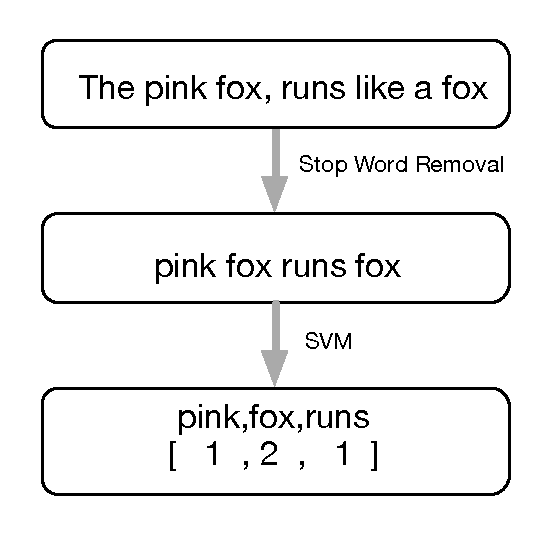
\includegraphics[width=5cm]{images/2_svm.eps}
  \end{center}
  \caption{ Text tokenization and transformation to Vector Space Model. }
  \label{fig:2_svm}
\end{figure}

There are many clustering algorithms. In the following section we will describe the particullar case of the \ac{SOM} algorithm, the solution used in our work.

\section{The Self-Organizing Map} 
\label{sec:the_self_organizing_map}

\ac{SOM} are a two layer recurrent \ac{ANN} that has the desired property of topology preservation, thus mimicking the way the cortex of highly developed animals brains work. \ac{SOM} allow cluster visualization of multi-dimensional data, similar to methods such as \ac{MDS}~\cite{KruskalWish1978} and \ac{PCA}~\cite{Hotelling_1933} .  

\citet{Bacao2005} described the basic idea behind \ac{SOM} as a mapping between input data patterns into a n-dimensional grid of neurons, or units. That grid is also know as the output space, as opposed to the initial space --- input space --- where the input patterns reside. An illustration of both spaces can be seen in Figure~\ref{fig:5_neighbours_converge}.

SOMs work in a similar way as is thought the human brain works. Analogously to the human brain, SOMs also have a set of neurons that, through learning experience, specialize in the identification of certain types of patterns. These neurons are responsible for categorizing the input patterns for which they are responsible to identify. Nearby neurons will be organized by similarity, which will cause similar patterns to activate similar areas of the \ac{SOM}.
With this topology preserving mapping, the \ac{SOM} organizes information spatially, where similar concepts are mapped to adjacent areas. The topology is preserved in a sense that, as far as possible, neighborhoods are preserved throughout the mapping process.
Output neurons are displayed in an N dimensional grid, generally rectangular, but other structures are possible, such as hexagonal or octagonal.  The grid of neurons, in the output space, can be divided in neighborhoods --- where neurons responsible for the same kind of input reside.
In \ac{SOM}, neurons will have the same amount of coefficients as the input patterns and can be represented as vectors.

Before describing the algorithm, it is important to define two key aspects of the \ac{SOM}: the learning rate and the quantization error. The learning rate is a function that will be decreased to converge to zero. It will be applied to winning neurons and their neighbors in order for them to move toward the corresponding input pattern in progressively smaller steps. Quantization error is the distance between a given input pattern and the associated winning neuron. It describes how well neurons represent the input pattern. The radius of the neighborhood around the winning neuron is also particularly relevant to the topology of the \ac{SOM}, deeply affecting the unfolding of the output space as stated by~\citet{Bacao2005}. 

SOM training is always subject to some variability due to multiple causes, like the sensitivity of initial conditions, convergence to local minima and sampling variability~\cite{Bodt}.

No general formula exists to minimize quantization error~\cite{Bodt} . In order to achieve a minimal value, the number of neurons, value of neurons and order of the input data is randomly changed. Multiple SOMs are trained and the one with the lowest mean quantization error is chosen.

In order to know how well a neuron maps to all the input patterns it represents, the average of the quantization error can be used(Eq. \ref{eq:avg_quant_error}). On the equation, $d_{i,n}$ is an input pattern that is represented by the neuron $w$. Each neuron represents an arbitrary number --$n$--of input patterns, that group of input patterns is represented as $D_{i,j}$.
\par
\begin{equation}
  \label{eq:avg_quant_error}
  \varepsilon(w) = \frac{\sum_{i=0}^{n} \| w - d_{i}  \| }{n}, d_{i} \in D, \forall n
\end{equation} 


\input{./algorithms/som.tex}


\begin{figure}
  \begin{center}
    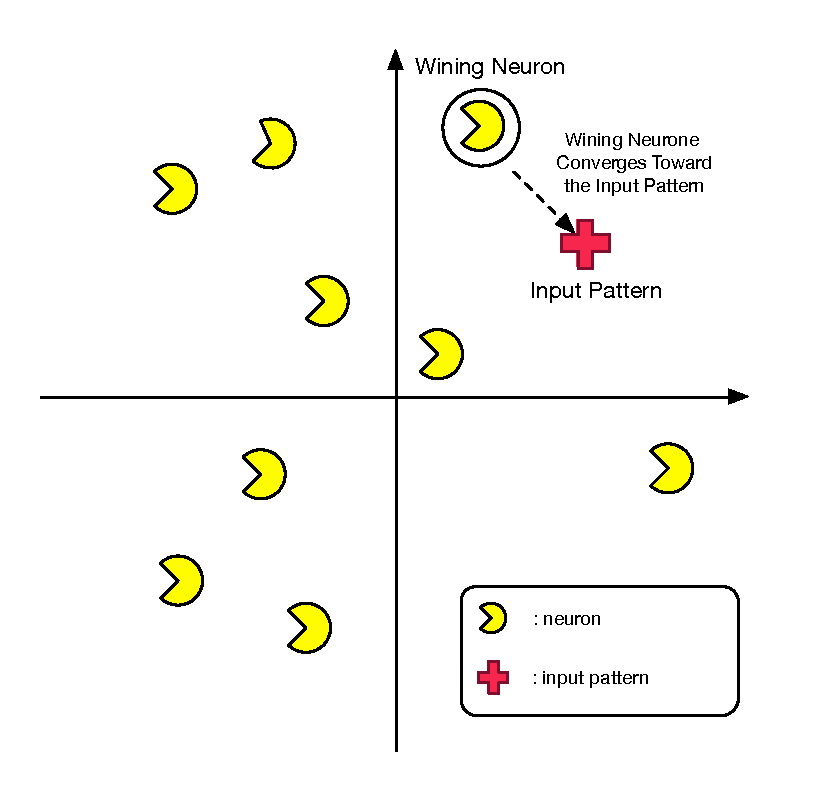
\includegraphics[width=5cm]{images/4_wining_neuron_converge.eps}
  \end{center}
  \caption{ Winning neuron converging at learning rate }
  \label{fig:4_wining_neuron_converge}
\end{figure}

\begin{figure}
  \begin{center}
    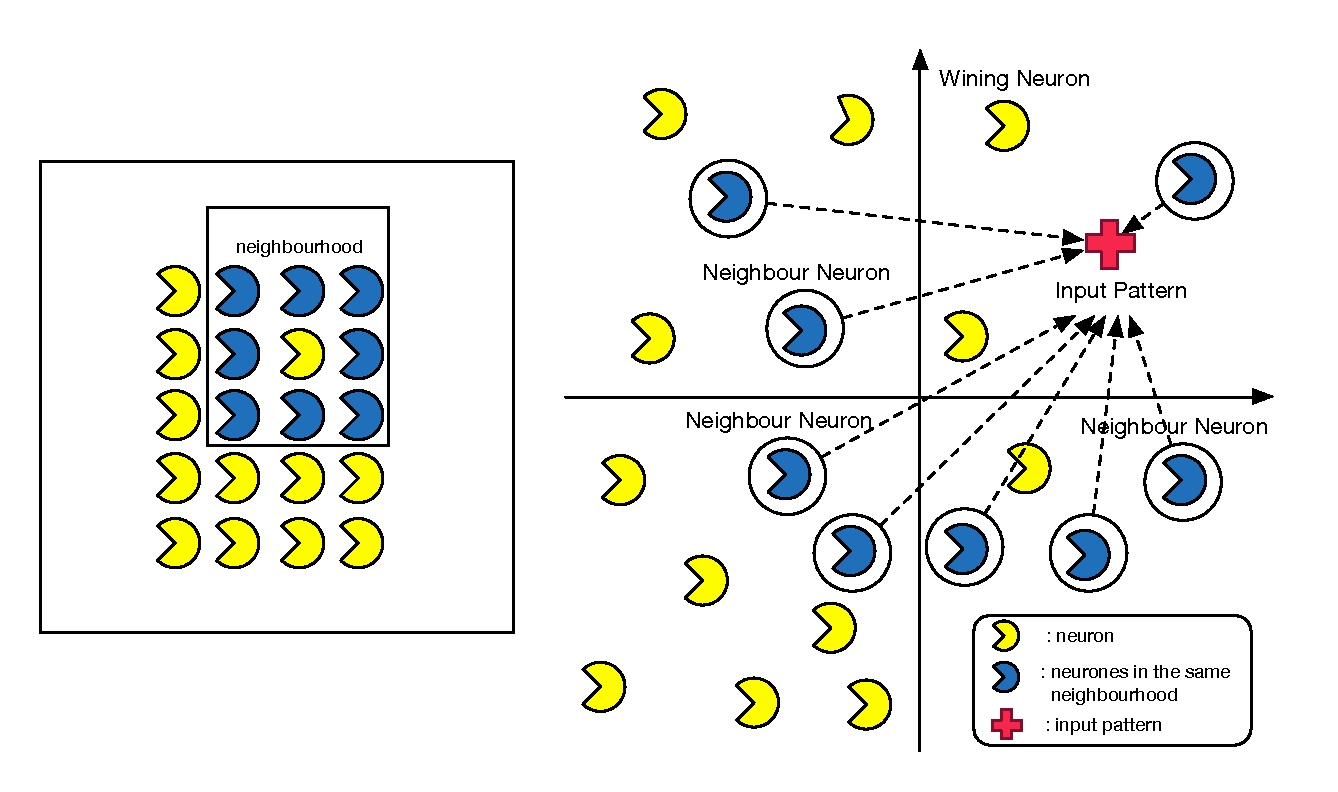
\includegraphics[width=12cm]{images/5_neighbours_converge.eps}
  \end{center}
  \caption{ On the left the output space neighborhood, on the right the neighbors of the winning neuron converging in the direction of the input pattern }
  \label{fig:5_neighbours_converge}
\end{figure}

The prediction phase can start after the model is learned. On the prediction phase, new input patterns can be quickly assigned to the \ac{SOM}, without need to apply the learning rate to the winning neuron and his neighbors. In other words, only line~\label{som:one} will run. Due to the fact that the input pattern will be assigned to the cluster that is mapped by the nearest neuron. Thus, it is very easy and fast to classify new data now. As stated by ~\citet{Liu2012b}, the advantages of using \ac{SOM} are: data noise immunity, easy to visualize data, and parallel processing.

In order to visually interpret the result of the \ac{SOM}, \ac{U-Matrix} method may be used~\citep{Bacao2005}. The \ac{U-Matrix} is a representation of the \ac{SOM}, in which, the distance between neurons is represented in a gray-scale where the darkest colors represent the farthest distance and the lightest colors the closer neurons. One way to compute the \ac{U-Matrix} is described in~\ref{alg:umatrix}. 

\begin{figure}[h]
  \begin{algorithm}[H]
    \label{alg:umatrix}
    \DontPrintSemicolon
    \KwData{$W = \{  \overrightarrow{w_{0,0}}$,\dots,$\overrightarrow{w_{n,n}}$ \} are the trained neurons 

            $D_{i,j}$ be the input patterns represented with neuron $w_{i,j}$

            $U$ is an empty matrix with size $2n-1.2n-1$
  }
    \KwResult{U-Matrix}
    \tcc{Initialize $U$ by adding the trained neurons}
    \For{ $w_{ij} = \overrightarrow{w_{00}}$ to $\overrightarrow{w_{n,n}}$ }{
      $U_{i*2, j*2} \leftarrow w_{i,j}$
    }
    \tcc{Calculate the distance between every adjacent neurons, and apply it to the square between them}
    \For{ $i=0$ to $U_{max}$}{
           
      \For{  $j=0$ to $U_{max}$}{
        
        \If{$l+1<m || j+1<m$}{
          $U_{i+1, j} = \| u_{i,j} - u_{i+2,j} \| $
          $U_{i, j+1} = \| u_{i,j} - u_{i,j+2} \| $
          $U_{i+1, j+1} = \frac{\| u_{i,j} - u_{i+2,j+2} \| + \|u_{i+2,j} - u_{i,j+2} \| }{2}$

        }
        $ j \leftarrow j + 1 $
      }
      $ i \leftarrow i + 1 $
    }
    \tcc{Substitute the neurons for an average of surrounding distances}
    \For{ $i=0$ to $U_{max}$}{
      \For{  $j=0$ to $U_{max}$}{
        $ u_{ij} = avg( Adj[u_{ij}] )$

        $ j \leftarrow j + 1 $
      }
      $ i \leftarrow i + 1 $
    }
    \tcc{convert the distances to color}
    $WHITE = 255$

    $BLACK = 0$

    $ u_{max} \leftarrow max(U) $

    $ u_{min} \leftarrow min(U) $

    \For{ $u_{ij} = u_{00}$ to $u_{n,n}$ }{
      $U_{i, j} \leftarrow (1 - \frac{ u_{i,j} - u_{min}  }{u_{max}-u_{min}})* WHITE$
    }
    \caption{U-Matrix }
  \end{algorithm}
\end{figure}


The \ac{U-Matrix} algorithm ( Alg.~\ref{alg:umatrix} ) is composed by four main cycles, which work in the following way:

\begin{itemize}
  \item \textbf{Cycle 1: } On line~\ref{um:initialize} neurons are added to the empty matrix, in order to be able to calculate the distance between them.
  \item \textbf{Cycle 2:} From line \ref{um:distance_h} to \ref{um:distance_d}, we are calculating the distance between adjacent neurons, and adding the distance to the empty position between them. On line \ref{um:distance_h} and line \ref{um:distance_v} we are looking for neurons horizontally and vertically, respectively. On line \ref{um:distance_d} we are looking for neurons on the diagonal. The diagonal calculus is more complex due to the fact that we need to calculate the lower diagonal to the current neuron, and average it withe the upper diagonal of the neuron immediately billow it.
    \item \textbf{Cycle 3: }At this stage the matrix is full of the distances between neurons, theoretically nothing else would be needed to be calculated. But it still has neurons residing on the matrix which need to be removed. On line \ref{um:rem_n} we substitute all neurons with an average of the distances surrounding them.
    \item \textbf{Cycle 4:}  Finally all the values on the matrix are substituted by colors on a black to white scale. Bigger distances between neurons are represented with darker colors while smaller distances are represented with lighter colors. This conversion is done on line \ref{um:conv_color}
  
\end{itemize}

An example of an \ac{U-Matrix} can be seen in Figure~\ref{chp3:img2}.

\begin{figure}[htpb]
  \centering
  \subfigure[SOM ouputspace trained with random RGB vectors]{\includegraphics[scale=2]{./images/som_training/2_som.pdf}\label{chp3:img1}}
  \hspace*{0.5cm}
  \subfigure[U-Matrix representing how well each neuron maps to input patterns it represents]{\includegraphics[scale=1.05]{./images/som_training/2_umatrix.pdf}\label{chp3:img2}}\\
  \caption{U-Matrix and SOM output space, computed after 300 epochs of training, with 1500 random input patterns representing an RGB color.}
  \label{fig:umatrix_and_ouputspace}
\end{figure}



\fancychapter{State of the art}
%\section{Related Work}
%\label{sec:related_work}

This Section provides insight of work done in multiple research areas that are related to the project. In subsection ~\ref{sub:self_organizing_maps} will be described multiple work done using Self-Organizing maps. Subsection ~\ref{sub:topic_detection_on_twitter} is dedicated to work done on topic detection on the social network Twitter \footnote{http://www.twitter.com}

\section{Self-Organizing Maps} 
\label{sec:self_organizing_maps}
Self-Organizing maps are used in a wide are of applications, from authentication systems~\cite{Dozono2012} through network intrusion detection ~\cite{intrusion_som} and speech recognition and analysis~\cite{phonetic_typewiter}.

\subsection{The Geo-Som} 
\label{sub:types_of_soms}
The Geo-SOM~\citet{Bacao2005} applies the first column of geography “Everything is related to everything else, but near things are more related than distant things." to the SOM algorithm, where the winning neuron is chosen in a radius defined by the geo-coordinates of the data, forcing units that are close in the input space to be close in the output space. The representation of the Geo-som can be seen in Figure ~\ref{fig:geo_som}.

\begin{figure}[tb]
  \begin{center}
    \includegraphics[]{images/6_geo-som.png}
  \end{center}
  \caption{Geo-SOM structure, from~\citet{Bacao2005}}
  \label{fig:geo_som}
\end{figure}

\subsection{Detecting Hidden Patterns on Twitter Usage} 
\label{sub:detecting_hidden_patterns_on_twitter_usage}
Cheon and Lee~\citep{Cheong2010} analyzed hidden patterns created the natural usage of twitter by its users. In its study they started by collecting data from the twitter API of different kinds of topics like "2009 Iran Election" and "iPhone 3.0 OS launch". They made multi level signal extraction not only from information directly present on the tweet, but also by cross referencing with other social website and with the twitter user profile information. The signals retrieved from the social network can be seen in Table ~\ref{tab:twitter_signals}.

\begin{table}[H]
  \caption{Twitter Signals}
  \label{tab:twitter_signals}
  \begin{center}
    \begin{tabular}{|l|}
      \hline
      \textbf{Twitt Corpus}  \\
      \hline
      Tweet Size \\
      \hline
      Replies \\
      \hline
      Re-tweets \\
      \hline
      Hashtags  \\
      \hline
      \specialcell{Presence of URIs and \\ Type of linked content} \\
      \hline
      Type of Device   \\
      \hline
      Tweet Location  \\
      \hline                 
      \hline                 
      \textbf{Twitter Profile} \\ 
      \hline
      Account Age   \\
      \hline
      Gender     \\
      \hline
      Country \\    
      \hline
      frequency of posts \\
      \hline
      Friends to followers ratio \\ 
      \hline
      Number of  customizations \\   
      \hline
      \hline
      \textbf{External Sources} \\
      \hline
      Other Social Network Accounts   \\
      \hline
      Type of website\\ 
      \hline
    \end{tabular}
  \end{center}
\end{table}

By applying a SOM, they could find 4 demographical clusters during the Iran 2009 Election. The first columnster was characterized by young web-based Iranians, with twitter accounts not older than 3 months with a high frequency of replies. The second cluster was mainly compound of web users from Iran accounts older that 3 months. The third cluster had Iranian users with mobile clients with large texts clearly trying to raise awareness. The fourth and final cluster represented the users around the world trying to raise awareness about the issue by sharing tweets with URIs.
Looking at their analysis about the topic "2009 Iranian Election" it is clear to see that it was possible to describe the type of users represented in the social network and the way they interact with it.

On the iPhone 3.0 OS launch it was possible to find three main clusters. The first columnster was characterized by male users, accounts older than 90 days, coming from countries where the iPhone is marketed, with high adoption of social media clearly representing the target market of the iPhone or its customers. The second cluster had new accounts with higher rate of followers to followees, high frequency of posts per day, presence of URI linking to technology blogs or websites, no country or gender specified meaning that this cluster was clearly composed by news aggregators and technological news websites. Inside the second cluster there was a sub-cluster of Japanese users which represents the high rate of iPhone adoption in Japan. Finally the third cluster was clearly spammer accounts that where eventually deleted after a couple of months, characterized by popular social connections, posting more than 50 tweets a day with external URIs and the accounts where not older than a day or so.

In conclusion it was possible to detect Twitter usage patterns and specifically detect spammers before they where banned from the social network. 

\section{Topic Detection and Clustering} 
\label{sec:topic_detection_on_twitter}
There have been many topic detection techniques. Many of them rely on the TF ID~\cite{Baeza-Yates:1999:MIR:553876} (term frequency – inverse document frequency) which is not particularly adequate for topic detection on Twitter due to the fact that tweets are very small, composed by typos or slang words and might be written in multiple languages, sometimes at the same time. In this subsection we will take a look at multiple methods of topic detection in general and specifically on the Twitter social network.

\subsubsection{Topic and Trending Detection} 
\label{ssub:real_time_topic_and_trending_detection}
Due to the rapid adaptation of people to always be on-line, through the usage of cellphones on the move, desktops at work and even theTV at home, the increase of user generated content has increased tremendously in latest years. In 2006 35\% of on-line adults and 57\% of teenagers created content on the Internet \footnote{ Data source: http://www.pewinternet.org/Presentations/2006/UserGenerated-Content.aspx}, which in "Internet Years" was ages ago.
With amount of content increasing, new real-time and scalable algorithms are needed in order to make sense of all this data.
~\citet{Cataldi2010} propose a new technique for emerging topic detection that permits real-time retrieval of the most emergent topics expressed by a community on Twitter. Their work applies the PageRank~\cite{Pagerank1998} algorithm to the users follower/followee relationship in order to find the most influential user on the network, and then calculates the most trending topics by relating, social influence, word co-occurrence and time frame. In the end, an interface was created where it would be possible to navigate hot topics in a given time frame. Topic labeling was not automatic and was implicit by the time frame of an event, if two highly social events would occur in the same time frame with word relations the results could be interpreted as the same, for example if a political candidate would win the elections at the same of an important sports club would win a specific cup, the word \emph{win} could be trending at the same time for two different topics and due to high temporal dependency they could be interpreted as the same topic.
~\citet{Weng2010} also used the PageRank algorithm in order to find the most influential twitter users on a certain topic, but uses a different approach where they represent each twitter user as a bag of words comprising of all the tweets that they have posted. Afterwards it uses Latent Dirichlet Allocation~\cite{Blei2003} in order to find the topics each user is interested in. In the end it was possible to prove that follower/followee relation on twitter was not just casual, but that people actually follow other people in which they have some resemblance or common interest. This concept is called homophily and will be further explored by this project.

\section{Twitter Data Mining} 
\label{sec:data_mining_in_twitter_}
In this subsection, we will focus on work done on the Twitter social network in order to leverage insights on how the public data available from the website can correlated within itself and with outside sources. 

\subsection{Tweets Hidden Data} 
\label{sub:the_tweet}
Tweet retrieval and analysis is a double edged problem. On one side the tweet is really small which makes it almost impossible to retrieve any actual sense from it. On the other hand the amount of tweets generated per day is around 140 million \footnote{https://blog.twitter.com/2011/numbers} wich means that it is very hard to a deep analyses of the semantics and content of individual tweets, and that, only the more appropriate signals should be evaluated.
~\citet{Tao2012} evaluated how the multiple signals that could be retrieved directly or indirectly from the tweet corpus could mean that a tweet is relevant for a determined topic. In his work, Tao presents premises that seem intuitively true and proves they actually are relevant through a comparison of multiple precision and recall values. Its results on feature comparison where summarized in Table ~\ref{tab:tao_table}, the first column consists of all the made hypothesis categorized by type, and the second column tells if the data used actually influenced in precision and recall results. Tau also compared result of topic characteristics, concluding that distinction between local and global events as well as temporal persistence proved to not be relevant on relevance prediction.

\begin{table}[tb]
  \caption{~\citet{Tao2012} tweet characteristics hypotesis versus influence}
  \label{tab:tao_table}
  \begin{tabularx}{\textwidth}{|X|l|}
  \hline
  \textbf{Hypotheses} & \textbf{Influence of Features} \\
  \hline
  \hline

  {\bf Syntatical} &  \\
  \hline
  Tweets that contain hashtags are more likely to be relevant than tweets that don't & Not Important \\
  \hline
  Tweets that contain an URI are more relevant that tweets that don't  &Important \\
  \hline
  Tweets that are replies to other tweets are less relevant & Important \\
  \hline
  The longer the tweet is the more relevant it is & Not Important\\
  \hline
  \hline

  {\bf Semantic}  &  \\
  \hline
  
  The more the number of entities the more relevant a tweet is  & Important \\
  \hline
  Different types of entities are of can have different amount of interest to a give topic  & Important \\
  \hline
  The greater the diversity of concepts mentions in a tweet the more likely for it to be relevant & Important \\
  \hline
  The relevance of a tweet is determined buy its polarity & Important \\
  \hline
  \hline

  {\bf Contextual} &  \\
  \hline
  The lower the temporal distance between a query and the creation of a tweet the more relevant the tweet is  & Not Important \\
  \hline
  The more the number of tweets created by a user the more relevant one of his tweets will be & Not Important \\
  \hline
  \end{tabularx}
\end{table}

~\citet{McCreadie2013} also approached the issue of having very little content on tweets in order to categorize a tweet, and tried to solve it by applying the content of linked URIs into the tweet body in order to improve precision and recall. The best fitting approach was using Field-Based weighting where for each tweet a new document is created which contains two fields; the terms in the tweet and the terms in the linked document. 
Afterwards a learning to rank algorithm called PL2F is used against the dataset from Microblog2011 in order to find the best weighting that should be applied to the tweet corpus and the URI referenced page. 
With this trained model they where able to improve precision in an order of 0.9, over only analyzing the text contained in the tweets. 

\subsubsection{Rapidly Changing Trends} 
\label{ssub:real_time_}
Due to the real time nature of Twitter, using typical retrieval model that relies on term frequency models like BM25 or language modeling cannot be applied, as stated by~\citet{Lin2012}. The study of topic perdurance on the social network proved that it is presented in bursts of queries and mentions of a topic. The typical usage of twitter for search is not the same of Google. When user are searching in twitter they want to find out what is happening right know meaning that classification techniques based on past events cannot respond this kind problem. As stated by~\citet{Lin2012} this problem has not yet been solved at Twitter (or anywhere else at the time of writing this report), and issues a new kind of data analysis approach that was not taken into consideration in the past. 
This effect of rapidly changing topics and queries based on real time events was named "Churn", and can be clearly seen in Figure ~\ref{fig:churn}.

  \begin{figure}[tb]
    \begin{center}
    \noindent\makebox[\textwidth]{
      \includegraphics[width=13cm]{images/7_churn.png}
    }
    \end{center}
    \caption{The Churn effect: Frequencies of queries related to Steve Jobs death over a 12 hour period in 5-minute intervals, normalized to the total number of queries in the interval. At its peak, the query “steve jobs” reaches 0.15 (15\% of the query stream); Graph taken from~\cite{Lin2012}}
    \label{fig:churn}
  \end{figure}


\section{Summary}
%TODO Sumarize the state of the art
Ending section summarizing the chapter is typically a good idea.

Ensure that the next chapter starts in a odd page
\cleardoublepage 

\fancychapter{Clustering Tweets with Self Organizing Maps}
\label{ch:clustering_tweets}

\section{Adapting the SOM to the Social Web}
\label{sec:adapting_the_som_to_the_social_web}

{\color{red} transform tweets in binary matrix's and train them }
Tweets categorization with \ac{SOMs} requires a dataset to work on. Due to systematic API restrictions, which where implemented in order to protect Twitter business model, gathering a dataset that directly maps to the social network is a great challenge by itself. 
In order to categorize tweets with \ac{SOMs} first we used a dataset provided by INESC-ID. The dataset had almost 1TB of data in \ac{JSON} format.

\section{Crawling Twitter for Social Relations}
\label{sec:crawling_twitter}
The INESC twitter dataset, was a good dataset to start analyzing the complexity of clustering tweets. On Chapter \ref{ch:clustering_tweets} we deeply analyzed the characteristics of the INESC twitter dataset, and concluded that it was not optimal to the problem we are trying to solve since it doesn't have the social connections between the authors of the tweets.

\section{SOM Framework}
{\color{red} Resume this section }

\subsection{Motivation}
\label{sec:motivation}
When researching ways to extend the \ac{SOM} algorithm, in order to add social features to the learning process. I found that the number of \ac{SOM} libraries was not very extense. Even though, programing languages often used in \ac{ML} and Data Mining, such as Python or C++, have their how implementation of the \ac{SOM} algorithm. I've found that most of these libraries are made in such a way to be extremely fast, in order to take as much advantage from the hardware they are running on as possible. They often lack the modularity needed to adapt the \ac{SOM} algorithm to specific problems.

The \ac{SOM} algorithm has been changed many times in order to better categorize data with specific features, for example Geo-SOM was described in Subsection~\ref{sub:types_of_soms}, the Growing Hierarchical SOM~\cite[]{1058070}, the time adaptive SOM~\cite[]{1187438}, the Ontological SOM~\cite[]{5446427}, and the list goes on\dots  

In order to create the homophilic SOM, described in Section~\ref{sec:algorithm_changes} we first created a SOM framework that is easy to extend due to be fully object oriented, scripted --- even though it can be compiled to run on the JVM --- and without C extensions.


\section{Clustering Socially Connected Data}
The default \ac{SOM} algorithm has no idea whatsoever of the social connections between the tweets, it simply looks at the binary vectors that represent sentences and assigns it to the most similar neuron.

In order to better categorize socially connected data, we propose some alterations to the \ac{SOM} algorithm in order to make it aware of the social connections between the tweets, and therefor better represent the homophilic behavior present on social networks.

{\color{red} insert homophilic som algorith here}

\section{Homophilic SOM Definition}
\label{sec:algorithm_changes}

\subsection{Output Space}
\label{sub:output_space}
The outputs space is the zone on the \ac{SOM} algorithm where the neurons reside. It works like a cortex where neurons are scattered in a geometric fashion, generally a square. The output space is generally initialized with random values, with a relatively high learning rate, and also a relatively high number of epochs. The algorithm is made this way in order to be able to identify any type of data that can be represented as vectors.

First we will try to change the output space to better resemblance the social network. In order to do this, the squared grid that defines the output space was changed by the social network connections, and the neurons, are represented by a social network user. This changes are applied in the following way:
\begin{figure}[htpb]
  \centering
  \subfigure[The neighbourhood is defined by the relations of followers/followees between the winning neuron and the other neurons]{\includegraphics[scale=0.3]{./images/homophilic_outputspace.pdf}\label{chp3:homout}}
  \hspace*{0.5cm}
  \subfigure[Homophilic input space works in the same way as a normal input space]{\includegraphics[scale=0.3]{./images/homophilic_input_space.pdf}\label{chp3:homin}}
  \label{fig:homo_in_out}
  \caption{ Homophilic SOM output and input space during the learning phase. }
\end{figure}
\begin{itemize}
  \item Each neuron is comprised of the text from all the tweets that he authored.
  \item Each neuron has a unique id, and stores the ids of his followers and followees that are present in the output space.
  \item During the learning phase, the radius will be defined as the maximum number of hops separating the winning neuron and followers/followees of followers/followees. 
  %\item Each neuron will cache followers/followees of a follower/followee to a specified depth level, for performance purposes. 
\end{itemize}

{\color{red} insert image of the output space with social features vrs tipical output space}

\subsection{Learning Phase}
\label{sub:learning_phase}
Like in the default \ac{SOM} the learning phase is where the output space is trained in order to organize the input data into clusters. Since this algorithm is specific to categorize tweets using social network features, the learning rate, radius and number of epochs used can be greatly reduced in order for the algorithm to converge. The learning phase operates in the following way:

\begin{itemize}
  \item The distance between the input pattern and all the neurons is calculated. The neuron closest to the input pattern is considered the winning neuron.
  \item When the winning neuron is selected, he and his social neighbors within k hops, update their representations in the input space, and move closer to the input patter. The Gaussian function (Func.~\ref{eq:gaussian}) is also used in here in order for the neighbors that are closer to the input pattern be significantly more influenced by the input pattern, while the neurons further away are less influenced. 
  \item This process is repeated for a predefined number of epochs. While the number of epochs increases, the learning rate, and number of hops that defines the neighborhood decreases in order for the algorithm to converge.
\end{itemize}

Just like the default \ac{SOM} algorithm, after the map is trained, input patterns can be fast assign to the nearest neuron since the neuron positions in the output space are no longer updated.

{\color{red} Link to the learning phase in the algorithm on the main chapter, add images of the training model }

\section{Social Clusters}
\label{sec:hmophilic_som_clusters}
{\color{red} resume what is written in this chapter }

\subsection{Training}
\label{sub:dataset}
In order to train the Homophilic SOM, we used the crawler defined in Section~\ref{sec:data_mining_in_twitter_}. The dataset had the following characteristics:
{\color{red} add table with number of users, tweets, tags, on the dataset}
{\color{red} show amount of time it took to train the SOM}
{\color{red} show umatrixes of the trainne }
{\color{red} compare clusters/time and umatrixes of the default SOM and the Homophilic SOM}
{\color{red} show the tweets in some clusters }



 \fancychapter{Implementation}
 %TODO how it was implemented
I have no idea what to write here\dots

\begin{figure}
\begin{boxedverbatim}
DefineGlobals
   clock   alias   clk
   reset   alias   rst
   max_latency     17
   feedback        0
   DefineInputs
      X   std_logic_vector(11 downto 0)
   EndInputs
   DefineOutputs
      Y   std_logic_vector(11 downto 0)
   EndOutputs
EndGlobals
\end{boxedverbatim}
\caption{An example code section.}
\label{chp4:img}
\end{figure}

Figure~\ref{chp4:img} shows an example of a \verb"\boxedverbatim" section. It allows to put blocks of code within a frame. I think makes a prettier printing.

\section{Summary}

An ending section summarizing the chapter, is typically a good idea.

% Ensure that the next chapter starts in a odd page
\cleardoublepage


\fancychapter{Evaluation Metrics}

\section{Clustering Tweets with Self-Organizing Maps}
\label{ch:clustering_tweets}

\subsection{SOM training}
\label{sub:clustering_tweets_with_soms}
Our first approach to cluster tweets with \ac{SOM} started by dynamically creating \ac{VSM} for each new word that was encountered while scanning each tweet. Due to simplicity of the approach, an overwhelming amount of different words, some, even without any clear meaning. 
Due to the huge amount \ac{VSM} size, the trainings at hand took an eternity to process, in order to prevent this from happening we took a sample of 50MB of tweets, all in English, from the dataset and started to train the \ac{SOM} with it. String manipulation for \ac{VSM} reduction described on Subsection~\ref{sec:reducing_som_vector_size} where used.
The \ac{SOM} training was performed using the R kohonen package~\cite{rsom}. We have added some information about this train on Appendix~\ref{ch:rsom_training}, three kinds of clusters where found. Clusters where no topic could be made sense of, clusters with a ton of tweets which had the same text and clusters that had more than one topic/no topics at all. An example of tweets presents in these clusters can be seen in Figures \ref{fig:cluster1}, \ref{fig:cluster2} and \ref{fig:cluster3}.   

\begin{figure}[h!]
  \centering
  \subfigure[Cluster without topics]{\includegraphics[scale=0.6]{./images/clutercluster.pdf}\label{fig:cluster1}}
  \hspace*{0.5cm}
  \centering
  \subfigure[Cluster with the iPad topic]{\includegraphics[scale=0.6]{./images/ipadcluster.pdf}\label{fig:cluster2}}
  \hspace*{0.5cm}
  \centering
  \subfigure[Cluster with the iPad topic]{\includegraphics[scale=0.6]{./images/facecluster.pdf}\label{fig:cluster3}}
  \caption{Three types of clusters}
\end{figure}

\subsection{Reducing SOM vector size}
\label{sub:reducing_som_vector_size}
In Subsection~\ref{sub:clustering_tweets} we introduced string reducer methods which enabled great \ac{VSM} reduction. On Figure~\ref{fig:plot_word_red} we can see the amount of words removed by each method alone, and by all methods combined --- column "All Methods"---. In order to build this graph, we applied each method independently to a sample of 902802 tweets.

\begin{figure}[htpb]
  \centering
  \includegraphics[width=0.8\linewidth]{./plots/svm/plot_wordcount.pdf}
  \caption{Amount of unique words present on dataset sample with 902802 tweets, based on the string word reduction technique applied.}
  \label{fig:plot_word_red}
\end{figure}

It is interesting to see that each method by itself doesn't remove a great amount of words. The method that removed more words by itself was "remove non letters" --- which removes every character that is not a letter ---, at an order of 33\%. On the other hand, the method "remove stop words" by itself removed only 400 of words. This was expected due to the fact that the full list of MySQL stop words used by this method only has 543 words. All methods combined where able to reduce the \ac{VSM} size in about 75\%.

String reduction techniques work directly with text and has no notion whatsoever of linguistic semantics. I Subsection~\ref{sub:tweeter_natural_language_processing} we presented a twitter \ac{NLP} libray which can be used effectively to understand the linguistic semantics used on twitter. 

By feeding the same dataset as used above to the library we where able to identify multiple types of words that can afterwards be considered relevant for~\ac{TDT}. On Figure \ref{fig:plot_word_red}, the red bars show the amount of words unique words found under a specific semantic tag, whilst in red we can see words tagged under the same category after applying string reduction techniques.

Due to the fact that we are trying to identify topics, most of the tagged words are of no use. We chose to use only common nouns, proper nouns and hashtags during the clustering process. By applying all these filters to the dataset sample, we have a \ac{VSM} reduction of about 90\%, from 1 204 743 different words to 132 861.

\begin{figure}[htpb]
  \centering
  \includegraphics[width=0.8\linewidth]{./plots/svm/plot_wordcount_nlp.pdf}
  \caption{Number of words tagged with Ark Tweet NLP. In red we can see the number of words unique words tagged in each category, while in blue we can see the amount of unique words, after applying string reduction techniques.}
  \label{fig:wordcount_nlp}
\end{figure}

\subsubsection{Identify Tweets language}
\label{ssub:identify_tweets_lang}
Twitter is a social network with users from every corner of the world, and due to this fact, tweets tend to be in a lot of different languages which complicates the process of clustering due to increasing the number of sining ms, idiomatic expression and results interpretation due to lack of knowledge of a specific language.  
In order to find a tweets language, it is possible to see the language that a user has on his twitter profile through the twitter API, but these are not always the same thing. Some times, users use their profiles on different languages that the language in which they issue their tweets.
Identifying tweets that where not in the English language was done through the usage of Ruby library called whatlanguage~\footnote{https://github.com/peterc/whatlanguage}, which tries to identify one language through Bloom Filters. Inside the tweet there is a field which identifies the user language, we found that x is not acurate. Removing tweets that weren't in the english language reduced the amount of different words in x and therefor will reduce the dimensional size of the \ac{SOM}.
In order to prove that the using the whatlanguage library in conduction with the language which users have on twitter will improve the overall percentage of English written tweets, we took a random sample of 100 tweets from our own dataset, and categorized it by hand. Afterwards we compared the results of using only the language on the tweet, using the language detection library and both. The results are summarized on Table~\ref{tab:mac_test}.  
\begin{table}[H]
  \caption{Tweets language detection summary }
  \label{tab:mac_test}
  \begin{center}
    \begin{tabular}{|c|c|}
      \hline
      Total amount of tweets gathered      & 87  \\
      \hline
      \hline
      Tweets with user language and tweet language in english      & 25  \\
      \hline
      Tweets with user language and tweet language not in english      & 7  \\
      \hline
      \hline
      Tweets tagged in english and tweet language was in english      & 8  \\
      \hline
      Tweets tagged in english and tweet language was not       & 0  \\
      \hline
    \end{tabular}
  \end{center}
\end{table}


Even though the sample is quite small, it was possible to understand that if both techniques where combined in order to detect the language of the tweet, the biggest problem which we could come across, would be to discard tweets that where not tagged as being in English, but in fact where. This is preferable, given that it easier to get more tweets in order to have English tweets, than constructing an \ac{VSM} with foreign terms.

\subsection{Conclusions}
\label{sub:conclusions}

\section{Twitter Crawler}
\label{sec:twitter_crawler}
After analyzing the work accomplished by clustering tweets with \ac{SOM} we decided that some alterations to the algorithm should done in order for it to take into account the fact we are dealing with socially connected data. In order to accomplish this we needed a dataset with social connections of behind the author of the tweet. There was two ways to accomplish this: 

\begin{itemize}
  \item \textbf{First aproach: } For each tweet we have on our dataset, fetch the user information including the users he is connected to.
  \item \textbf{Second aproach: } Create our own crawler, where the social connections, tweets and users are saved.
\end{itemize}                                                                                             
We followed the second approach in order to have more control over the data used from this moment forth, and to have a better integration of the tweets with the \ac{SOM} framework, described in Section~\ref{sec:som_framework}.

When designing the twitter crawler, we took into consideration that it had to be extremely resilient in order to be able to be left alone, crawling the twitter, until told to stop. Also if anything happened to the machine where the crawler was running it would be necessary to return to some previous crawling state, with minimum data loss. The crawler works in the following way:

\begin{itemize}
  \item \textbf{Step 1:} Choose some seed users to start crawling or deserialize a serialized version of the crawler if available.
  \item \textbf{Step 2:} For each seed user get all of his followers, and add them to an array if they haven't yet been crawled.
  \item \textbf{Step 3:} Repeat step one with random users taken from the array on step 2, until API limit is reached.
  \item \textbf{Step 4:} When API limit is reached, print the state of the crawled network, serialize the current state, and wait 15 minutes until it is possible to resume crawling. 
\end{itemize}

The crawler is able to get an average of 3 users with their social connections, and 150 tweets per 15 minutes window, it serializes itself to \ac{YAML} which besides being directly compatible with Ruby, it is also human readable making it easy to parse with unix tools.


\section{SOM Framework}
\label{sec:som_framework}
The \ac{SOM} framework was developed in the Ruby programing language \footnote{https://www.ruby-lang.org/en/} due to the desired characteristic of allowing great levels of introspection and being an almost pure object oriented programing language. Due to this characteristics making modifications to core parts of the algorithm is fairly easy.

The \ac{SOM} Framework was developed in a test driven fashion, having 100\% of its public methods tested and documented for expected behavior. These characteristics, associated with the fact that was published under an open source license, makes it available for other researchers to implement their own SOM variants.

By default, the base SOM algorithm is implemented as described by the Algorithm~\ref{alg:som} in Section \ref{sec:the_self_organizing_map}. 
\subsection{Clustering Color Vectors}
\label{sub:main_features}
Out of the box, the \ac{SOM} Framework implements a squared output space, where all residing neurons are manipulated as arrays. It is possible ate any given moment of the training to export the output space to \ac{JSON}, \ac{CSV} or to visualize its current \ac{U-Matrix}. Also during training a progress bar is displayed in order to know how much time will be needed for the training to end.

Due to the features described above, it is possible to train a \ac{SOM} to identify random colors --- RGB vectors --- while printing the results. In order to do this we will start by:
\begin{itemize}
  \item Initializing a SOM object with an output space size of 15 by 15 neurons, which will yield a total of 255 neurons --- and directly maps to the maximum number of clusters --- and 700 epochs.
  \item Create 1500 input patterns with size 3 and random values between 0 and 255. 
  \item Tell the SOM to print its state at the end of each epoch.
\end{itemize}
The machine used for training had the hardware specifications outlined in table \ref{tab:mac_test}.

\begin{table}[H]
  \caption{Test machine one specs}
  \label{tab:mac_test}
  \begin{center}
    \begin{tabular}{|c|c|}
      \hline
      Operative System & OSX 10.9.5 \\
      \hline
      Memory           & 8 GB, 1067MHz DDR3       \\
      \hline
      Processor        & 2,4GHz Intel Core 2  Duo \\
      \hline
      Hard Drive       & 128GB SSD  \\
      \hline
    \end{tabular}
  \end{center}
\end{table}


A summary of the training is specified in Table~\ref{tab:som_colours}
\begin{table}[H]
  \caption{SOM trainning resumed}
  \label{tab:som_colours}
  \begin{center}
    \begin{tabular}{|c|c|}
      \hline
      \textbf{Number of Neurons} & 225 \\
      \hline
      \textbf{Output Space Size} & 15x15 \\
      \hline
      \textbf{Number of Input Patterns} & 1500 \\
      \hline
      \textbf{VSM size of Input Patterns and Neurons} & 3 \\
      \hline
      \textbf{Number of Epochs} & 600 \\
      \hline
      \textbf{Training Duration} & 14 hours \\
      \hline
      \textbf{Type of Train} & print each epoch training\\
      \hline
      \textbf{Initial learning rate} & 0.6\\
      \hline
      \textbf{Initial Radius} & 8\\
      \hline
    \end{tabular}
  \end{center}
\end{table}


\begin{figure}[h!]
  \includegraphics[scale=0.6]{./plots/som/topological_error.pdf}
  \label{fig:top_error}
  \caption{Changes in topological error throughout the SOM training, lrate stands for learning rate, and radius for radius applied to the winning neuron}
\end{figure}

On Figure~\ref{fig:top_error} we can see the evolution of the topological error and how it is converging throwout the training process, as the radius and learning rate are decreasing, and as well as the number of epochs is rising. 

\begin{figure}[h!]
  \centerline{\includegraphics[scale=0.6]{./plots/som/average_distance.pdf}}
  \label{fig:avg_dist}
  \caption{Changes in the average distance between neurons, throughout the SOM training}
\end{figure}

On Figure~\ref{fig:avg_dist} we can see the average distance between neurons increasing. At first this might not look like a desired property, but in fact it is. When the distance between the neurons is increasing and the topological error is decreasing, it means that the neurons are scattering in the output space in order to better identify the input patterns they are responsible for.

During the training of this \ac{SOM}, we analyzed the output space, \ac{U-Matrix} and \ac{Q-Matrix} during the begging, half of the train, and finally at the end of the training.
When comparing the output space on Figure~\ref{onesom} at the staring of the training, it is possible to see a lot less colors that on Figure~\ref{threesom}, this is due to the fact that neurons are getting more specified through the training. 
The \ac{U-Matrix} evolves in a way where clusters are almost unnoticeable, which is due to the fact that each neuron is a cluster by itself, and the distance between it and his neighbors was homogenized throughout the output space. 
The \ac{Q-Matrix} evolves, by becoming whiter which represents that the mean topographic error is becoming smaller. This was already seen before in Figure~\ref{fig:top_error}, but now we can also see which neurons are worst at representing the input patterns.  

\begin{figure}[h!]
  \centering
  \subfigure[Output Space]{\includegraphics[scale=1]{./images/som_training/1_som.pdf}\label{chp3:onesom}}
  \hspace*{0.5cm}
  \subfigure[U-Matrix]{\includegraphics[scale=0.5]{./images/som_training/1_umatrix.pdf}\label{chp3:onematrix}}
  \hspace*{0.5cm}
  \subfigure[Q-Matrix]{\includegraphics[scale=1]{./images/som_training/1_quantmatrix.pdf}\label{chp3:onetopmat}}
  \hspace*{0.5cm}
  \caption{ SOM state after first epoch of training. Its learning rate is at 0.598, and radius at 8.  }
  \label{fig:}
\end{figure}

\begin{figure}[h!]
  \centering
  \subfigure[Output Space]{\includegraphics[scale=1]{./images/som_training/2_som.pdf}\label{chp3:onesom}}
  \hspace*{0.5cm}
  \subfigure[U-Matrix]{\includegraphics[scale=0.5]{./images/som_training/2_umatrix.pdf}\label{chp3:onematrix}}
  \hspace*{0.5cm}
  \subfigure[Q-Matrix]{\includegraphics[scale=1]{./images/som_training/2_quantmatrix.pdf}\label{chp3:onetopmat}}
  \hspace*{0.5cm}
  \caption{ SOM state after second epoch of training. Its learning rate is at 0.22, and radius at 3.  }
  \label{fig:}
\end{figure}

\begin{figure}[h!]
  \centering
  \subfigure[Output Space]{\includegraphics[scale=1]{./images/som_training/3_som.pdf}\label{chp3:threesom}}
  \hspace*{0.5cm}
  \subfigure[U-Matrix]{\includegraphics[scale=0.5]{./images/som_training/3_umatrix.pdf}\label{chp3:threematrix}}
  \hspace*{0.5cm}
  \subfigure[Q-Matrix]{\includegraphics[scale=1]{./images/som_training/3_quantmatrix.pdf}\label{chp3:threetopmat}}
  \hspace*{0.5cm}
  \caption{ SOM state after third epoch of training. Its learning rate is at 0.081, and radius at 1.  }
  \label{fig:}
\end{figure}

In order to see how well the neurons are representing the input patterns, we looked at the \ac{Q-Matrix} and selected the darkest area in order to know which neuron is the worst at representing its input patterns. Afterwards we printed the input patterns associated to that neuron. This process was graphically represented in Figure~\ref{fig:somtrained} where the colors which represent the input patterns are in fact RGB vector coordinates used during training. It is possible to see that even though this neuron ought to be the worst at representing it input data, he represents it quite well as they are all shades of red. 
It is important to know that all of this visualization can only be made due to the fact that, we are working with arrays with three dimension and values comprised between 0 and 255 which makes it possible for them to be presented as RGB images. 

\begin{figure}[h!]
  \centering
  \includegraphics[width=0.8\linewidth]{./images/som_trainned.pdf}
  \caption{Input patterns associated with the neuron with maximum topological error --31. Even though the neuron has the biggest topological error of all neurons, it still has a good representation of the input patterns. The colors in this image are not figurative, and represent the entities at the end of training  }
  \label{fig:somtrained}
\end{figure}

\subsection{Benchmarking}
\label{sub:benchmarking}
The \ac{SOM} was not created with the purpose of being extremely fast, for that there are already very goo implementations like \citet{somoclu} distributed library for \ac{SOM} or \citet{rsom} R kohonen package which implements the training algorithm in C, and only exposes the interface in the high level language R.  
Being purely written in a higher level language, the \ac{SOM} framework enables researchers and programmers to write training algorithms very fast. For example the code necessary for training the colored vectors on the previous Subsection can be seen in Figure~\ref{fig:rubysom}.

\begin{figure}[h!]
  \centering
  \begin{boxedverbatim}
  ## Create a new SOM object
  som = SOM::SOM.new output_space_size: 15, epochs: 1500

  ## Generate 1500 random input patterns
  som.input_patterns = 1500.times.inject([]){ |arr| arr << Array.new(3){ rand(0..255) }; arr  }

  ## Start training
  som.exec!
  \end{boxedverbatim}
  \caption{ Ruby code necessary for training a SOM with 1500 input patterns.  }
  \label{fig:rubysom}
\end{figure}

In order to better understand the amount of data \ac{SOM} framework is able to handle, we benchmarked it on the same machine used in Table~\ref{tab:mac_test}. The framework was tested against multiple sizes of output space and input patterns, multiple numbers of input patterns, and multiple numbers of epochs. 
The results where summarized on Figure~\ref{fig:benchmarkingsom}, where it is possible to see on the upper quadrant that if all parameters increase, \ac{SOM} training will suffer as well.

\begin{figure}[h!]
  \centering
  \includegraphics[width=0.8\linewidth]{./plots/som/benchmarking.pdf}
  \caption{SOM framework train duration, influenced by output space size in the x axis, number of epochs in the left, size of input patterns on top, and number of input patterns on the right in color from red to blue.}
  \label{fig:benchmarkingsom}
\end{figure}


\section{Homophilic SOM}
\label{sec:homophilic_som}

In order bring the concept of homophily --- love of the same --- to clustering socially connected data, on Section \ref{sec:algorithm_changes} we suggested some alterations to the default \ac{SOM} algorithm. These alterations where mainly applied to the output space of the \ac{SOM}, where in order for the neurons to actually represent users, and the connections between users of a social network. 

These features where implemented into the \ac{SOM} framework described in the previous chapter. The data used to train the homophilic \ac{SOM} can be seen in Table \ref{tab:homosom}. The training was performed on a machine with the characteristics show in Table \ref{tab:acer_test}.

\begin{table}[H]
  \caption{Second test machine specs}
  \label{tab:acer_test}
  \begin{center}
    \begin{tabular}{|c|c|}
      \hline
      Operative System & Ubuntu 13.10\\
      \hline
      Memory           & 16GB DDR3 Synchronous 1600 MHz      \\
      \hline
      Processor        & Intel(R) Core(TM) i7-3770 CPU @ 3.40GHz \\
      \hline
      Hard Drive       & 2TB HDD  \\
      \hline
    \end{tabular}
  \end{center}
\end{table}

\begin{table}[H]
  \caption{Homophilic SOM characteristics}
  \label{tab:homosom}
  \begin{center}
    \begin{tabular}{|c|c|}
      \hline
      Number of tweets & 1575 \\
      \hline
      Number of users & 25  \\
      \hline
      Output space size        & 100 \\
      \hline
      Input space size       & 3342 words  \\
      \hline
      Words used for clustering & Hashtags, comon and proper nouns  \\
      \hline
      SVM reductors used & all  \\
      \hline
      Training duration & 74h \\
      \hline
      Initial number of hops & 4 \\
      \hline
    \end{tabular}
  \end{center}
\end{table}


It is not possible to draw a \ac{U-Matrix} due to the fact that the output space from is no longer a rectangular matrix, but a graph. Also drawing the \ac{Q-Matrix} is possible, but the disposition of the neurons will not represent the actual disposition in the graph. This can still be useful to easily visualize which neurons are better at representing their input patterns. 

Looking at the results, there are a lot of different topics of clusters. There where neurons clearly responsible to identify music, like it can be seen on Figure~\ref{clust:tech}. On Figure~\ref{clust:music} we can see a cluster about tech and programing, the most surprising part about this cluster is that the tweet about the banana phone, is actually inserted into the tech topic --- it was tech project presented at codebits ---. 
On the other hand, some clusters of people saying that they have posted photos on facebook, or that they've liked youtube videos where also found. Even though they can be considered topics, their relevance is not very high.

\begin{figure}[h!]
  \centering
  \subfigure[Cluster about tech and programing]{\includegraphics[scale=0.6]{./images/1clustertech.pdf}\label{clust:tech}}
  \hspace*{0.5cm}
  \centering
  \subfigure[Cluster about music]{\includegraphics[scale=0.6]{./images/2clustertech.pdf}\label{clust:music}}
  \label{fig:clusters}
  \caption{Two clusters with different topics}
\end{figure}

\section{Conclusions}

% Ensure that the next chapter starts in a odd page
\cleardoublepage
 %\subsection{Twitter Dataset}
%\label{subsec:twitter_dataset}

%As can be seen in Figure~\ref{fig:json_tweet_user} no information about the social relations of the user which emitted the tweet are present. Therefor in order to retrieve the social network in which a user is contained, it will be necessary to connect to the Twitter API. Crawling twitter is discussed in further depth in Chapter~\ref{chap:crawling_twitter}.  


%In order to better understand the dataset at hand, all the \ac{JSON} files where converted into \ac{CSV}in a way to reduce the size of the dataset. While tweets where being converted, \ac{URL} where removed --- since most of them where minified in order to fit in less that 140 characters, without translating the minified URL, not a lot of information can be gathered. Also, all tweets that where not identified as being in English where also removed. The tweet shown in \ac{JSON} format in Figure~\ref{fig:json_tweet} is converted to \ac{CSV} in Figure~\ref{fig:csv_tweet}.
 
%%%%%% REMOVED STUFF
%\subsection{Topology Preservation} 
%\label{sub:topology_preservation}
%The Self-Organizing Map performs a mapping from the n-dimensional input space into the two dimensional output space and where resides one the most fascinating characteristics, which is that the output map tries to preserve the topology from the input space. This grants the SOM algorithm a way to visualize high-dimensional data that other neural networks or clustering algorithms don't have. Even though this is true, sometimes during training it is not possible to preserve the topology of the network.
%Thus topology preservation can be measured through the Topographic error~\citet{Kiviluoto1996} which is the proportion of all data vectors for which first and second BMUs \footnote{unit that is closest to the winning neuron. BMU Best fitting unit } are not adjacent units.
%In this project the Topographic Error will be calculated for all SOM implementations and VSM usages in order to understand if the representation of the SOM output space is well defined.

 %\begin{itemize}
  %\item show UMatrixes and multiple steps map trainning of the SOM library trainnig
  %\item show metrics for the crawller, tweets per second, users persecond, size of the dump a long the time.
  %\item compare my som library with other som libraries: training velocity with diferent parameters, map after trainned.
  %\item Compare Homophilic-SOM results with non homophilic: UMatrixes, cluster results, Quantization error, jacknife. 
%\end{itemize}
%%\section{Evaluation Metrics} 
%%\label{sec:evaluation_metrics}
%Evaluation of the topic detection on Tweets will be made in two distinct ways. The first way will focus on  binary classification using the precision and recall metrics, and will be described in Subsection~\ref{sub:testing_for_precision_and_recall}. The second way will focus on statistically testing the SOM learning process and the computed trained network. This testing process will be described in Subsection~\ref{sub:cluster_quality_testing}. 

%\section{Testing for Precision and Recall} 
%\label{sec:testing_for_precision_and_recall}
%Precision and Recall are both ways to measure the rate of right guesses made by the trained SOM network, and are defined in the following way:
%\begin{itemize}
  %\item \textbf{Precision:} Fraction of retrieved instances that where relevant 
    %\begin{equation}
  precision = \frac{|{relevant\;documents}\cap{retrieved\;documents}|}{{retrieved\;documents}}
\end{equation} 

  %\item \textbf{Recall:} Fraction of relevant instances that where retrieved
    %\begin{equation}
  recall = \frac{|{relevant\;documents}\cap{retrieved\;documents}|}{{relevant\;documents}} 
\end{equation} 

%\end{itemize}
 
%In order to calculate Precision and Recall we need to have the \emph{relevant documents} and the \emph{retrieved documents}. The \emph{relevant documents} are rather hard to determine because they need to be categorized by humans, which is an expensive task.

\fancychapter{Conclusions and Future Work}
Draw your conclusions here and sell your work. Trasmit to the juri how hard it was to develop the presented work.

A future work section is usually here.

% Ensure that the next chapter starts in a odd page
\cleardoublepage
 


\pdfbookmark[0]{Bibliography}{bib}
\bibliographystyle{apalike}
\bibliography{bibliographies/library,bibliographies/sites}
\cleardoublepage   
\appendix
% %%%%%%%%%%%%%%%%%%%%%%%%%%%%%%%%%%%%%%%%%%%%%%%%%%%%%%%%%%%%%%%%%%%%%%
% First appendix
% %%%%%%%%%%%%%%%%%%%%%%%%%%%%%%%%%%%%%%%%%%%%%%%%%%%%%%%%%%%%%%%%%%%%%%
\fancychapter{Appendix A}
\cleardoublepage

% %%%%%%%%%%%%%%%%%%%%%%%%%%%%%%%%%%%%%%%%%%%%%%%%%%%%%%%%%%%%%%%%%%%%%%
% Second appendix
% %%%%%%%%%%%%%%%%%%%%%%%%%%%%%%%%%%%%%%%%%%%%%%%%%%%%%%%%%%%%%%%%%%%%%%
\fancychapter{Appendix A}
\cleardoublepage  

\end{document}
